\documentclass{article}
\usepackage{exercise}
\usepackage[obeyspaces]{url}
\usepackage[dvipsnames]{xcolor}
\usepackage{graphicx}
\usepackage{listings}
\usepackage[scaled]{helvet}
\usepackage{amsmath,amssymb,amsfonts,mathtools,cancel}

% typeset in helvetica
\renewcommand*\familydefault{\sfdefault}


% QE stuff
\def\qe{{\sc Quantum ESPRESSO}}
\def\pwx{\texttt{pw.x}}
\def\cpx{\texttt{cp.x}}
\def\phx{\texttt{ph.x}}
\def\nebx{\texttt{neb.x}}
\def\configure{\texttt{configure}}
\def\PWscf{\texttt{PWscf }}
\def\PHonon{\texttt{PHonon}}
\def\CP{\texttt{CP}}
\def\PostProc{\texttt{PostProc}}
\def\NEB{\texttt{PWneb}} % to be decided
\def\make{\texttt{make}}
%%%%%%%%%%%%%%%%%%%%%%%%

\def\ipi{i-PI}
\newcommand{\hints}[1]{\emph{Hints: #1}}
\newcommand{\lstinxml}{\lstinline[language=XML]}
\newcommand{\lstinbash}{\lstinline[language=Bash]}
\usepackage[space=true]{accsupp}

\newcommand{\pdfactualhex}[3]{\newcommand{#1}{%
\BeginAccSupp{method=hex,ActualText=#2}#3\EndAccSupp{}}}

% PASTABLE lstlisting code
\pdfactualhex{\pdfactualdspace}{2020}{\textperiodcentered\textperiodcentered}
\pdfactualhex{\pdfactualsquote}{27}{'}
\pdfactualhex{\pdfactualbtick}{60}{`}

\lstset{tabsize=4,basicstyle=\ttfamily,breaklines=true,columns=flexible,emptylines=10000}
\lstset{literate={'}{\pdfactualsquote}1
                 {`}{\pdfactualbtick}1
                 {\ \ }{\pdfactualdspace}2
}

\lstset{
    basicstyle=\ttfamily,
    keywordstyle=\color{BrickRed},
    commentstyle=\color{Gray},
    stringstyle=\color{black},
    emphstyle=\color{RedOrange},
    columns=flexible,
    showstringspaces=false,
    xleftmargin=1em,
    deletekeywords={bin,all}
}


\lstdefinelanguage{Bash}
{
   alsodigit={-,.},
   morekeywords={ cp2k.popt, lmp_ubuntu, i-pi, vmd, for, done, python, mpirun, touch, tail, trajworks, autocorr, awk, i-pi-mergebeadspdb, grep, head, cp, cd, cat, ls, pwd, bash, sed, mkdir, vi, sh}
   %morecomment=[s][\color{orange}]{#}{\}
}

%\lstdefinelanguage{Python}
%{
%    morecomment=[s][\color{orange}]{#}{\}
%}


\lstdefinelanguage{XML}
{
  morestring=[b][\color{RedOrange}]",
%  morestring=[s]{>}{<},
  morecomment=[s]{<?}{?>},
  morecomment=[s][\color{orange}]{<!--}{-->},
  identifierstyle=\color{BlueViolet},
  keywordstyle=\color{ForestGreen},
  stringstyle=\color{RedOrange},
%  tagstyle=\color{Blue},
  morekeywords={xmlns,version,type, mode, units, forcefield, filename, stride, overwrite, nbeads,prefix}% list your attributes here
}

\lstdefinestyle{XML}
{
\tagstyle=\color{Blue}
}

\title{An introduction to \ipi{}}
\author{Riccardo Petraglia, Michele Ceriotti}
\date{January 2017}

\setlength\parindent{0pt}

\begin{document}

\maketitle

% INTRO
In this set of exercises we will learn about the basics of \ipi\ and
its use jointly with \qe.

As may be already clear, \ipi\ is not meant to compute forces. Thus,
an external engine is needed. Once the external engine is set, \ipi\
takes care of the generation of the MD trajectory. This approach
is extremely flexible. For example different kind of forces can be
mixed within \ipi\ permitting the use of forces coming from different
sources: correcting terms from different software (\PWscf~+ external
dispersion correction) or multiple time step approaches with
expensive/cheap forces computations (see the Ring Polymer Contraction
method).

\begin{figure}[h!]
\centering
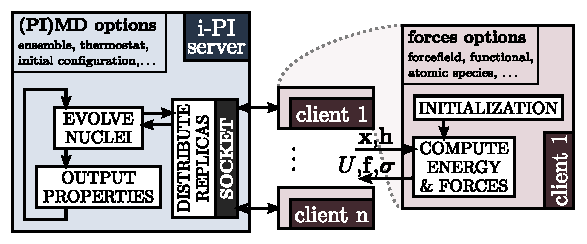
\includegraphics[width=0.9\textwidth]{ipi-scheme.pdf}
\caption{\ipi\ communicates with the force engine using sockets in a
  client/server fashion where \ipi\ behaves as the server. The engine
  connects to the server and provide \ipi\ the data it asks
  for.}\label{fig:ipi-scheme}
\end{figure}


The following exercises are created to increase the confidence of the user
with the \ipi\ workflow and to clarify the server/client approach on
which the \ipi-engine communication protocol is based (see
fig. \ref{fig:ipi-scheme}). Moreover, you will understand how to
set-up a simulation using the PIGLET thermostat to improve the Path
Integral Molecular Dynamics efficiency.


If you are using the VirtualBox image, all exercises are in the
sub-folder of \texttt{~/i-PI tutorial/exercises}. The folders with the
\texttt{-run} suffix contain the files resulting from the
tutorials. If you have doubts on how to proceed, having a look at
those files can be helpful.

\begin{Exercise}[label={i-pi},title={PIMD: a client/server approach}]

In this exercise, we will perform a simple Path Integral Molecular
Dynamics (PIMD) 
calculation using \PWscf\ as engine. Since the computation of QM forces is
expensive, here we use a single molecule of water in gas phase. Moreover, the
\PWscf\ input is prepared sacrificing the accuracy to run faster.

The simulation will be performed using the NVT ensemble at 300K.  We
will also record the kinetic and potential energy and the conserved
quantity of the system and the positions of the atoms.

\Question
Read the \PWscf\ input file \url{ex-1/pw.in}.
Is there any difference compared to a plain single point computation?
How is \pwx\ told where to find the \ipi\ server?\\

The input of \pwx\ is a valid input to run a single point
computation. To make \pwx\ aware of \ipi, you should specify an option argument
when starting the software (see section 3.6 of PWscf user's
manual).\newline

\vspace{1em}
\textbf{DO NOT RUN THE FOLLOWING COMMAND NOW!}
\vspace{1em}
\begin{lstlisting}[language=bash]
pw.x --ipi host:port < pw.in
\end{lstlisting}
The forces are then computed by \pwx\ at the level of electron theory
specified in the input and passed to \ipi\ thought the socket
interface.

\Question
Copy the \ipi\ input file \url{ex-1/ipi-template.xml} in
\url{ex-1/ipi.xml} and open the latter. Specifying in 
the input the address of the socket where \ipi\ will wait for a \pwx\
instance is essential. You have two possibilities: using a UNIX-domain
or an INET-domain socket. The former is faster but the server and the
client(s) must run on the same machine. The latter allows communication
through the ``internet'' so that \ipi\ and the ``force
calculator'' can run on a different computer.

The following steps tell \ipi\ to wait for a client connecting on the UNIX
socket called \texttt{single-water-qe}. Look for the following snippet
in the \url{ex-1/ipi.xml}:
\begin{lstlisting}[language=xml]
<ffsocket name="..." mode="unix">
<address>...</address>
</ffsocket>
\end{lstlisting}
Edit the file replacing the dots with appropriate values. Any string
would be fine, but if you
want to be consistent with the rest of the tutorial, you should use
the following:
\begin{table}[h!]
  \centering
  \begin{tabular}{ccc}
    \texttt{name} & $\longrightarrow$ & \texttt{pw-forces}\\
    \texttt{address} & $\longrightarrow$ & \texttt{single-water-qe}
  \end{tabular}
\end{table}


\textbf{Pay attention that attribute's values must be within single- or
double-quotes!}\\


The \texttt{name} attribute in the \texttt{<ffsocket>} node assigns a
reference to the forcefield within the \ipi\ input. This reference
will be used to specify the origin of the force within the
\texttt{<system>} node. If we want to use ``INET'' sockets, beside the
\texttt{<address>} node we have to provide a \texttt{<port>} node.


\Question
Introduce a \texttt{<force>} node that references to the previously
 defined \texttt{<ffsocket>}.

\ipi\ can manage different simulations at the same time. Each
simulation is defined in the \texttt{<system>} node. Each
\texttt{<system>} can also use forces coming from different
calculators. Since this is an introductory course, we are going to use
a single system with a single force. In the file \url{ex-1/ipi.xml}
look for the following snippet:
\begin{lstlisting}[language=xml]
<forces>
<force forcefield='...'/>
</forces>
\end{lstlisting}
Replace the three dots with the name of the forcefield you want to use
to compute the forces in this system. If you used the names suggested
in the tutorial, it should be \texttt{pw-forces}.

\Question
We are now ready to run the simulation.\\

The first thing to do is to start the \ipi\ server. Use the following
command when in the folder \url{ex-1}:
\begin{lstlisting}[language=bash]
$i-pi ipi.xml
\end{lstlisting}%$
If everything is fine, the shell will show some messages and will stop
with the following string:
\begin{lstlisting}[language=bash]
Created unix socket with address single-water-qe
@ForceField: Starting the polling thread main loop
\end{lstlisting}
this means that the server started correctly and is waiting for a
client that computes forces.

To start \pwx\ as an \ipi\ client open a new terminal, enter the
folder \url{ex-1} and \textbf{create a new directory}. \textbf{Enter this new folder} and run the
following command after replacing the \texttt{unix\_address} with the
actual address where \ipi\ is waiting (if followed tutorial
suggestions, this should be \texttt{single-water-qe}):
\begin{lstlisting}[language=bash]
$pw.x --ipi unix_address:UNIX < ../pw.in
\end{lstlisting}%$
When we use a UNIX socket, there is no need for specifying a port. The
\texttt{port} field, as shown in the first point of this exercise, is
then replaced by the \texttt{UNIX} string that tells \pwx\ to use a
UNIX socket. \\

\textbf{Optional}\\
If you have time, after finished the tutorial, you can
try using an INET socket. Define the address of the machine
where \ipi\ is running as \texttt{<address>} of the
\texttt{<ffsocket>} node. If also the client will run on the same
machine, you can use \texttt{localhost} otherwise, if the connection
between \ipi\ and the client uses internet, use as \texttt{<address>}
the actual IP address of the machine. The port can be any integer
in the range 15000-45000. When you start the client, remember to
modify the address and the port to match the ones used within the \ipi\
input.

\Question
Now switch to the terminal where \ipi\ is running, notice
that \ipi\ has built the connection with \pwx:
\begin{lstlisting}[language=sh]
 @SOCKET:   Client asked for connection from . Now hand-shaking.
 @SOCKET:   Handshaking was successful. Added to the client list.
\end{lstlisting}
and started the Molecular Dynamics simulation.
It should also dump out information on the time cost of each MD step
and about which \pwx\ instance is used (you can have more than one)
from each replica (bead).

\Question
Try to kill the \pwx\ instance.  Simply switch to the
terminal where \pwx\ is running and press \url{Ctrl+c}.  Now look at
whether \ipi\ is still running.  Notice that although the evolution of
MD is paused, \ipi\ itself does not die off but instead it continues to
run and wait for new client to take over.  Now start \pwx\ again using
the previous command.
What happens to \ipi\ now?  \ldots Nice eh?


\Question
What if one stops \ipi ?  Kill \ipi\ by typing \url{Ctrl+c}
where it is running, or create a file named \url{EXIT} in the folder
where \ipi\ is running (you can use the bash command \texttt{touch
  EXIT}).  Watch how \ipi\ responds, and how \pwx\ reacts.  Think
about what are the advantages of a clean exit when a MD program stops
unexpectedly. When \ipi\ dies cleanly, it generates a \texttt{RESTART}
file on the working directory. You can use that \texttt{RESTART} as a
valid input for \ipi. If look inside the file you can find all the
nodes that are also defined in the initial input. Beside them, you
also have many nodes to specify the status of the various quantities
when \ipi\ died.


\Question
Checking the \texttt{<initialization>} node in the \ipi\ input, we see
the attribute \texttt{nbeads=4}. This means that we are running a Path
Integral Molecular Dynamics (PIMD) simulation with 4 beads.
This explains why \ipi\ is producing so many xyz files as output. There
is an output for each bead and a fifth file containing the trajectory
of the centroid. You can open them all together with the following
command:
\begin{lstlisting}[language=bash]
vmd -m example*.xyz
\end{lstlisting}
You can also look at the \url{ex-1/example.out} file. This is the
result of the \texttt{<property>} node. The header of the file
summarizes what is printed in each column. You can create a graph using
the following command:
\begin{lstlisting}[language=bash]
plot example.out -1,3
\end{lstlisting}
The \texttt{-1,3} keyword tells to the script to use the column 1 as
x-axis and the column 3 as y-axis. You can discover more option simply
writing \texttt{plot} and pressing enter.
\end{Exercise}
\vspace{1em}

Before starting with the next exercise, stop the simulation (exiting
from \ipi\ as shown above) and  take a few minutes to explore
all the other keywords in the \ipi\ input. If you are familiar with
pother MD software, you should find the input quite self-explanatory.
Try to focus also on the \texttt{<output>} node and understand why
\ipi\ is printing all those files.


When you are tired of looking at a single molecule of water, go to the
next exercise.

MD simulations are quite computationally expensive and performing
simulation with \emph{ab-initio} force evaluation would require much
more time than you have during this tutorial. This is why,
from now on, the code LAMMPS will be used instead of \qe. All the
input for \qe\ will be present anyway in the exercise \texttt{-run} folders.

\vspace{2em}

\begin{Exercise}[label={inputs},title={Liquid water with the
    \emph{PIGLET} thermostat}]
In this exercise you are going to learn how to perform a PIMD
simulation using the PIGLET thermostat to improve the efficiency of
the sampling.

\Question
To start the exercise, perform the following steps:
\begin{itemize}
\item Copy the folder \url{ex-2} in \url{ex-2-piglet}.
\item  Enter the new folder, copy the file \texttt{ipi-template.xml}
  to \texttt{ipi.xml}. 
\item Open the new file and locate the node describing the
  thermostat (it is called \texttt{<thermostat>}).
\end{itemize}
The attribute \texttt{mode} of the
thermostat is set to \texttt{piglet}. The PIGLET thermostat requires
some parameters that can be downloaded from the following website
\url{https://epfl-cosmo.github.io/gle4md/index.html?page=matrix}.
To obtain the correct parameters for water do the following:
\begin{enumerate}
\item Select \texttt{PIGLET} as \textbf{GLE type};
\item Set the number of beads \textbf{N. beads} to \texttt{6};
\item The \textbf{Par. set} should be \texttt{Ns=8,
    $\hbar\omega/kT=20$, PIGLET}
\item To get the output in the \ipi\ input form, select \ipi\ in the
  \textbf{Output format}.
\item All the other parameters are left to the default value.
\end{enumerate}
In this context, the \texttt{Ns} are the number of degrees of freedom
of the bath, $\omega_{max}$ and \texttt{centroid} are the maximum
and the window frequencies for which the sampling is
enhanced. \textbf{Target T} is the temperature of the simulation and
$\hbar\omega/kT$ is the ratio between vibrational energy and average
kinetic energy.

\Question 
Use the following command to run the PIGLET/PIMD simulation with
\ipi:
\begin{lstlisting}[language=bash]
$i-pi ipi.xml
\end{lstlisting}%$

At this point you have two choices for the force provider: you may start
\PWscf\ or LAMMPS. Since this simulation contains 96 atoms, we warmly
suggest using LAMMPS in this test by running the following command
\begin{lstlisting}[language=bash]
$lmp_serial -i in.water
\end{lstlisting}%$
in a different shell. Keep this simulation running until the end of
the tutorial.

\Question
Run an MD simulation using a White Noise Langevin (WNL) thermostat.
Make a copy of the folder
\url{ex-2} and call it \url{ex-2-langevin}. Enter this latter, make a
copy of \url{ipi-template.xml} to \url{ipi.xml} and open this latter.
Replace the PIGLET thermostat (all the \texttt{<thermostat>} node:
from \texttt{<thermostat>} to \texttt{</thermostat>}) with the
following snippet:
\begin{lstlisting}[language=xml]
<thermostat mode='langevin'>
<tau units='femtosecond'>100</tau>
</thermostat>
\end{lstlisting}
Moreover, since we want to run a classical MD (not PIMD), set the
value of the attribute \texttt{nbeads} into the \texttt{<initialize>}
node to 1.

Since each socket must be unique, the value of the \texttt{<address>}
node must be changed: this one is already in use by the previous \ipi\
instance. Replace the \texttt{<address>} value with \texttt{ex2-2} and
start the \ipi\ server with the usual command:
\begin{lstlisting}[language=bash]
$i-pi ipi.xml
\end{lstlisting}%$

Before starting the LAMMPS instance we need to change the address
inside the LAMMPS input file. Open a new terminal, move to the
\url{ex-2-langevin} folder and open the file \url{in.water}. Locate
the line relative to \ipi. You can find it toward the end of the
file. Replace the value of the address (\texttt{ex2-1}) with the new
one: \texttt{ex2-2}. Now start the LAMMPS simulation with the already
known command:
\begin{lstlisting}[language=bash]
$lmp_serial -i in.water
\end{lstlisting}%$


While the simulation is running, in order to
understand the \ipi\ machinery better, you could prepare a \pwx\ input
for this example starting from the \pwx\ input provided in the folder
\url{ex-1/pw.in}. Try also to run it with \ipi\ to be sure it's
working (remember that you will have to change the socket address if
it is already used).\\
\vspace{2em}
\textbf{Do not stop the simulations of exercise 2!}


% \Question
% Stop LAMMS (press \url{Ctrl+c} in the terminal where it has been
% ran). \ipi\ is now waiting for a new connection. Restart LAMMPS with
% the following command:
% \begin{lstlisting}[language=bash]
% lmp_serial -i in.water > lmp.out.1 &
% \end{lstlisting}
% The shell should still present you the prompt. Run the same command a
% second time replacing the last ``1'' with a ``2''. What is happening
% in the \ipi\ terminal? You can see that now \ipi\ prints out much more
% information. Can you understand what they are? How many instances of
% LAMMPS could be used to maximize the performances?

\end{Exercise}

With this second exercise we performed a much more interesting
simulation using some advanced method to increase the efficiency of
the PIMD statistical sampling. Before moving to the next exercise, we
strongly suggest to run the same simulation using a white noise Langevin
thermostat and a single bead (classical dynamics).  Let both run while
working on the next exercise. We will come back to these at the end of
the tutorial to analyze some results.

At this point, you should know \ipi\ well enough to
proceed with the next simulation without much help. Pay attention to
the fact that only one instance of \ipi\ can use a given socket at
time. If you want to run two \ipi\ server at the same time, make sure
they have a different \texttt{<address>} or, in the case of INET domain
sockets, at least different \texttt{<port>}. At the end, you can look
at the differences between the two trajectories.

\vspace{2em}

\begin{Exercise}[label={inputs},title={PIMD-NPT simulation of ice}]
The goal of this exercise is to run a PIMD simulation in the NPT
ensemble. The \ipi\ input provided with the file \url{ex-3/ipi.xml} is
a valid input for a PIMD-NVT simulation. The idea is to transform it
in a valid input for a PIMD-NPT simulation.

\Question
Take a look at the input provided and identify the nodes responsible
for the task \ipi\ will perform.
\texttt{motion} is the most important node in this case.
Look at the following snippet:
\begin{lstlisting}[language=xml]
<motion mode='dynamics'>
<dynamics mode='nvt'>
<thermostat mode='langevin'>
<tau units='femtosecond'> 100 </tau>
</thermostat>
<timestep units='femtosecond'> 0.25 </timestep>
</dynamics>
</motion>
\end{lstlisting}
This section of the input tells \ipi\ that the computation we want to
perform is a molecular \texttt{dynamics}, in the \texttt{nvt} ensemble
using a \texttt{langevin thermostat} and a \texttt{timestep} of 0.25
femtosecond.

There is also another important section:
\begin{lstlisting}[language=xml]
<ensemble>
<temperature units='kelvin'> 200 </temperature>
</ensemble>
\end{lstlisting}
This node of the input define all the ensemble properties. In the
case you want to perform an NPT simulation, the pressure must be
defined within the \texttt{ensemble} node.


\Question
Add a barostat. You can follow the user guide to understand how to
set-up the barostat. Anyway, the following snippet provide a general setup
which is suitable for this case.
\begin{lstlisting}[language=xml]
<barostat mode='isotropic'>
<tau units='femtosecond'> 200</tau>
<thermostat mode='langevin'>
<tau units='femtosecond'> 100</tau>
</thermostat>
<h0> [ 25.6156, 0, 0, 0, 29.5783, 0, 0, 0, 27.8867 ]</h0>
</barostat>
\end{lstlisting}
Where is the place for this node? The \texttt{barostat} is a
characteristic of the \texttt{dynamics} itself. Then it must be
specified within that node. Copy the snippet aforementioned and paste
just before the \texttt{<timestep>} node.


\Question What if we want to perform an NPT simulation with an
anisotropic barostat? This kind of simulations need an extension of
the NPT ensemble, called NST (constant-temperature,
constant-stress). Thus, in \ipi\ set the attribute \texttt{mode} of
the \texttt{dynamic} node to \texttt{nst}. This means also that the
\texttt{<ensemble>} node must contain a stress tensor instead of an
isotropic pressure. To simulate our system with an anisotropic cell at
atmospheric pressure, use the following snippet inside the
\texttt{<ensamble>} node:
\begin{lstlisting}[language=xml]
<stress units='megapascal'> [10, 0, 0, 0, 10, 0, 0, 0, 10] </stress>
\end{lstlisting}
The stress is a 3x3 tensor. To simplify user's life, this kind of tensors are
flatten in the \ipi input.

At this point the input is ready to perform a simulation with at
``constant anisotropic pressure''.

\Question
What does the list \texttt{h0} contains? Why do we need a thermostat
within the barostat?

The list of numbers is a reference cell for the Parrinello-Rahman
barostat (which is the one implemented in \ipi). In practice, those
numbers are the dimension of the cell that must be written into the xyz
input file (\url{ex3-1/init.xyz}) or in the pdb file (take as an
example the one at \url{ex1/h2o-init.pdb}). The coordinate files
also contains the units of dimension of the cell and the positions
(\texttt{cell\{angstrom\}} and \texttt{position\{angstrom\}}).

\Question
Following the same procedure used in the last exercise, start this
simulation.

\end{Exercise}

\begin{Exercise}[label={inputs},title={Radial distribution function comparison}]
As a last exercise, you should compare the radial distribution
function obtained from the two simulation of exercise 2.

\Question
Compute radial distribution functions for the different simulations. You
can use any tool of your liking, but we suggest the \url{trajworks}
post-processing tool that is part of the \url{toolbox} library.
Run the following command in the two folders used during the exercise
2: \url{ex-2} and \url{ex-2-piglet}.
\begin{lstlisting}[language=bash]
$read_box <(tail -q -n +100 example.pos_*.xyz) > box.dat%$
$tail -q -n +100 example.pos_*.xyz | trajworks -ixyz \
        -box box.dat -gr -gr1 O -gr2 O -grmax 5 -grbins 250 -hwin \
        triangle  -hwinfac 2 > gOO.dat%$
\end{lstlisting}

To visualize the result you can use the \texttt{plot} command from
\url{ex-2-piglet} folder:
\begin{lstlisting}[language=bash]
plot gOO.dat ../ex-2-langevin/gOO.dat -1,2
\end{lstlisting}
Also compute the O--H radial distribution function.
Do you see any difference? Can you explain why?

\end{Exercise}

We hope this tutorial made you familiar with the use of \ipi. You
can find more tutorials and more information (as well as a link to the
last development and stable versions at \url{http://ipi-code.org}.


%\bibliographystyle{unsrt}
%\bibliography{biblio}
\end{document}
